%! Author = vova
%! Date = 26.09.2020

% Preamble
\documentclass[12pt]{article}

% Packages
\usepackage{amsmath}
\usepackage{romannum}
\usepackage{hyperref}
\usepackage{graphicx}
\usepackage{setspace}
% \usepackage[margin=1.0in]{geometry}

\title{On non-ideal voltage and current measurement tools}
\date{26.09.2020}
\author{Latipov Vladimir \&\& Onishenko Sergiy}


% Document
\begin{document}
    \pagenumbering{gobble}
    % \thispagestyle{empty}

    \doublespacing
    \doublespacing

    \maketitle
    \newpage
    \pagenumbering{arabic}

    \tableofcontents

    \newpage

    \section{Abstract}\label{sec:abstract}
    The contents of this section should be too abstract for me to be able to write it.

    \section{Experiments}\label{sec:experiments}
    There were 4 experiments arranged:

        \subsection{Experiment \textnumero1: Sequential plugging in}\label{subsec:experiment-1} % \Romannum{1}
    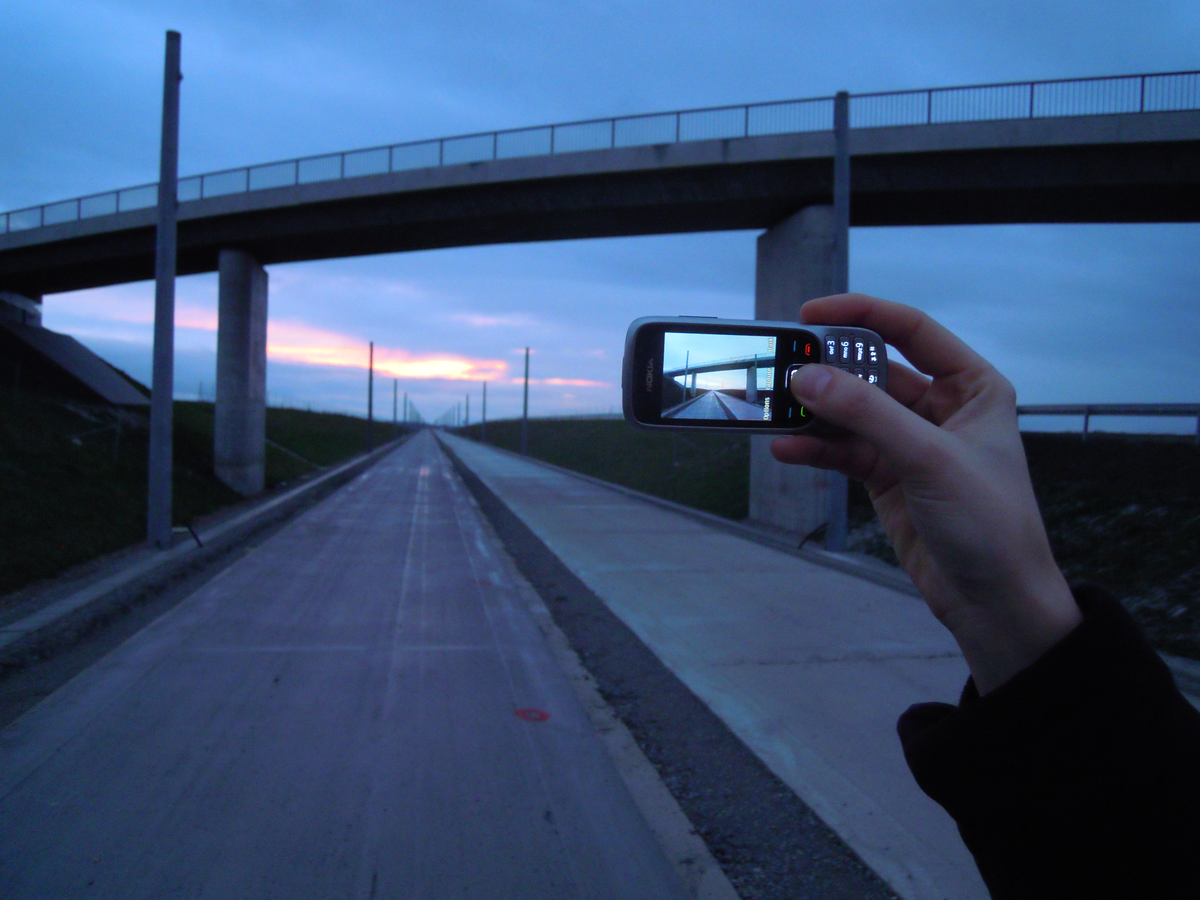
\includegraphics[width=\linewidth]{images/schemes/scheme0.png}

    \subsection{Experiment \textnumero2: Only Voltmeter}\label{subsec:experiment-2}
    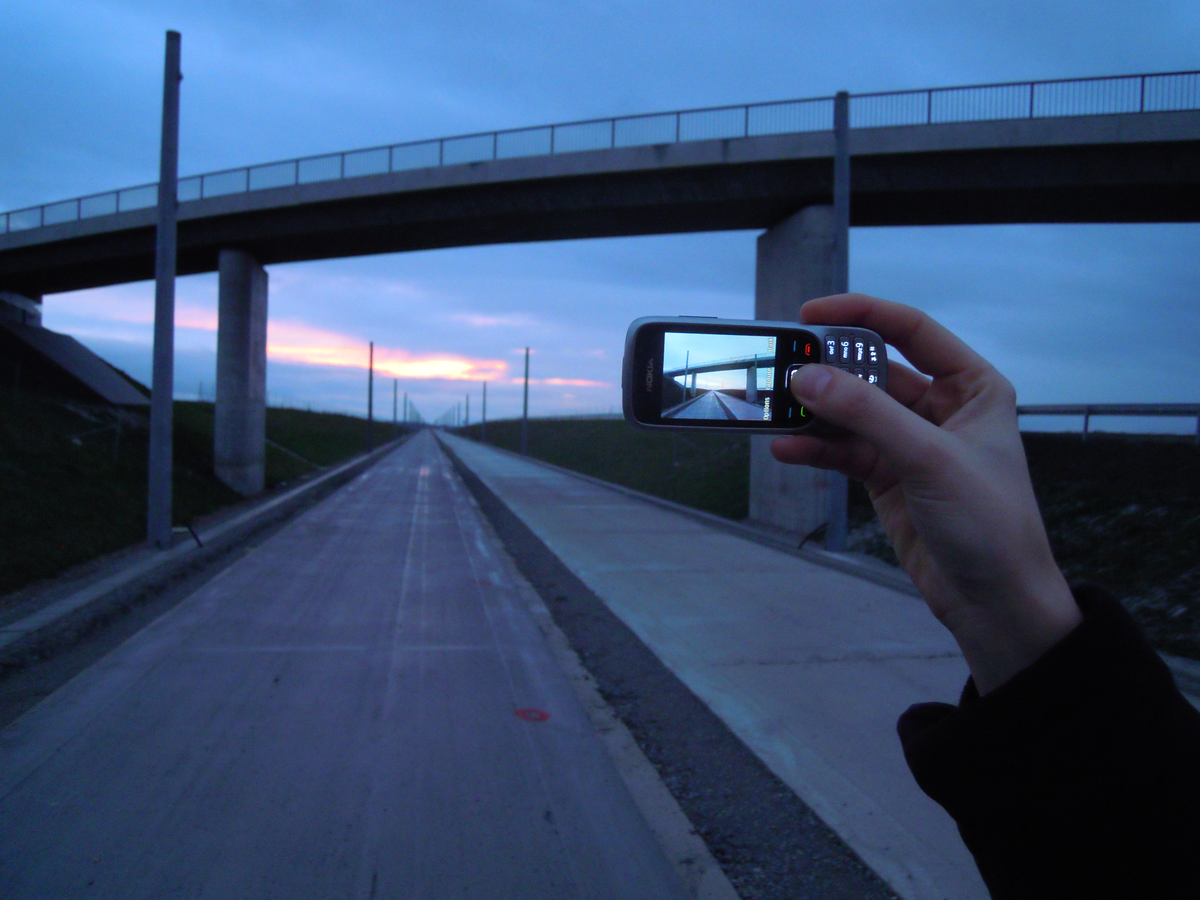
\includegraphics[width=\linewidth]{images/schemes/scheme0.png}

    \subsection{Experiment \textnumero3: Only Ampermeter}\label{subsec:experiment-3}
    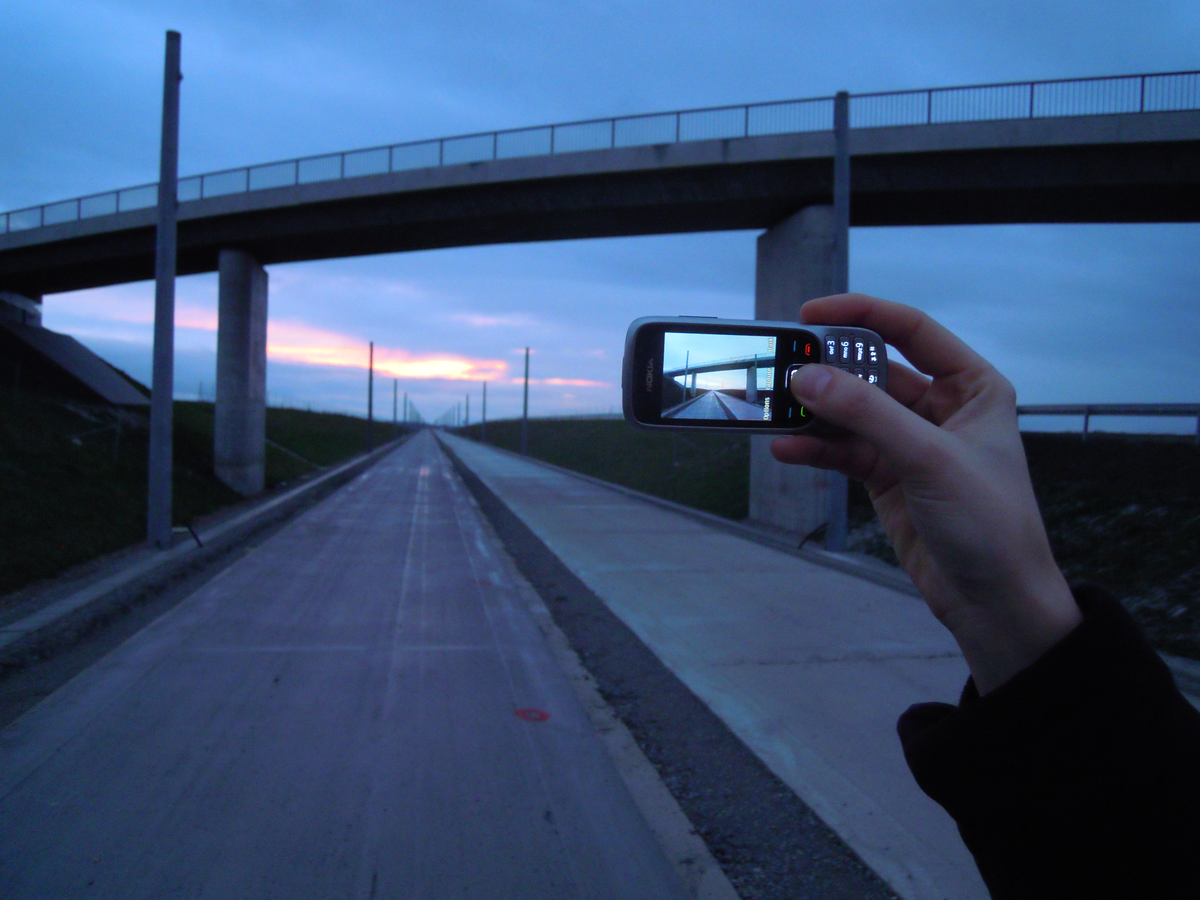
\includegraphics[width=\linewidth]{images/schemes/scheme0.png}


    \section{Solving equation system}\label{sec:solving-equation-system}

    \underline{\textit{\textbf{Some bold, italic and underlined text here}}}

    \begin{equation}
        A_1 = \frac{\varepsilon}{R_{all}}\label{eq:equation1}
    \end{equation}

    \begin{equation}
        V_1 = \varepsilon \cdot \frac{R_v}{R_{all}}\label{eq:equation2}
    \end{equation}

    \begin{equation*}
        R_v = \frac{V_1}{A_1}
    \end{equation*}

    \begin{equation}
        V_2 = \varepsilon \cdot \frac{R_v}{R_v + R_\varepsilon}\label{eq:equation3}
    \end{equation}

    \begin{equation*}
        \varepsilon = V_2 + V_2 \cdot \frac{R_\varepsilon}{R_v}
    \end{equation*}

    \begin{equation}
        A_3 = \varepsilon \cdot \frac{1}{R_A + R_\varepsilon} = \left(V_2 + V_2 \cdot \frac{R_\varepsilon}{R_v}\right) \cdot \frac{1}{R_A + R_\varepsilon} \label{eq:equation4}
    \end{equation}

    \begin{equation*}
        A_3 \cdot R_A + A_3 \cdot R_\varepsilon = V_2 + R_\varepsilon \cdot \frac{V_2}{R_v}
    \end{equation*}

    \begin{equation*}
        R_\varepsilon \cdot \left( A_3 - \frac{V_2}{R_v} \right) = V_2 + A_3 \cdot R_A
    \end{equation*}

    \begin{equation*}
        R_\varepsilon = \frac{V_2 + A_3 \cdot R_A}{A_3 - \frac{V_2}{R_v}}
    \end{equation*}

    \begin{equation*}
        \left(\ref{eq:equation1} \right) \rightarrow A_1 = \frac{\varepsilon}{R_{all}} = \frac{\varepsilon}{R_v + R_A + R_\varepsilon} = \frac{\varepsilon}{R_v + R_A + \frac{V_2 + A_3 \cdot R_A}{A_3 - \frac{V_2}{R_v}}} = \frac{\varepsilon}{R_v + \frac{V_2}{A_3 - \frac{V_2}{R_v}} + R_A \cdot \left( 1 + \frac{A_3}{A_3 - \frac{V_2}{R_v}} \right)}
    \end{equation*}

    \begin{equation*}
        \varepsilon = V_2 + V_2 \cdot \frac{\frac{V_2 + A_3 \cdot R_A}{A_3 - \frac{V_2}{R_v}}}{R_v} = V_2 + V_2 \cdot \frac{\frac{V_2}{A_3 - \frac{V_2}{R_v}} + \frac{A_3 \cdot R_A}{A_3 - \frac{V_2}{R_v}}}{R_v} = V_2 + \frac{V_2^2}{R_v \cdot A_3 - V_2} + R_A \cdot \frac{A_3 \cdot V_2}{A_3 \cdot R_v - V_2}
    \end{equation*}

    \begin{equation*}
        V_2 + \frac{V_2^2}{R_v \cdot A_3 - V_2} + R_A \cdot \frac{A_3 \cdot V_2}{A_3 \cdot R_v - V_2} = A_1 \cdot R_v + \frac{V_2 \cdot A_1}{A_3 - \frac{V_2}{R_v}} + R_A \cdot A_1 \cdot \left( 1 + \frac{A_3}{A_3 - \frac{V_2}{R_v}} \right)
    \end{equation*}

    \begin{equation*}
        R_A \cdot \frac{A_3 \cdot V_2}{A_3 \cdot R_v - V_2} - R_A \cdot A_1 \cdot \left( 1 + \frac{A_3}{A_3 - \frac{V_2}{R_v}} \right) = A_1 \cdot R_v + \frac{V_2 \cdot A_1}{A_3 - \frac{V_2}{R_v}} - V_2 - \frac{V_2^2}{R_v \cdot A_3 - V_2}
    \end{equation*}

    \begin{equation*}
        R_A \cdot \left( \frac{A_3 \cdot V_2}{A_3 \cdot R_v - V_2} - A_1 \cdot \left( 1 + \frac{A_3}{A_3 - \frac{V_2}{R_v}} \right) \right) = A_1 \cdot R_v + \frac{V_2 \cdot A_1}{A_3 - \frac{V_2}{R_v}} - V_2 - \frac{V_2^2}{R_v \cdot A_3 - V_2}
    \end{equation*}

    \begin{equation*}
        R_A = \frac{A_1 \cdot R_v + \frac{V_2 \cdot A_1}{A_3 - \frac{V_2}{R_v}} - V_2 - \frac{V_2^2}{R_v \cdot A_3 - V_2}}{\frac{A_3 \cdot V_2}{A_3 \cdot R_v - V_2} - A_1 \cdot \left( 1 + \frac{A_3}{A_3 - \frac{V_2}{R_v}} \right)}
    \end{equation*}

    \begin{equation*}
        R_\varepsilon = \frac{V_2 + A_3 \cdot R_A}{A_3 - \frac{V_2}{R_v}}
    \end{equation*}

    \begin{equation*}
        \varepsilon = V_2 + V_2 \cdot \frac{R_\varepsilon}{R_v}
    \end{equation*}




    \section{Measurement Results}\label{sec:measurement-results}

    We`re neglecting the inaccuracy of the pre-determined upper device measurement limit which is written on those devices.
    It`s inaccuracy is pretty low!

    \begin{equation*}
        A_1 = \left( \left(0.6 \pm 0.07 \right) Ampere \right) \times \frac{15.8}{2000} = \left(4.7 \pm 0.6 \right) milliAmpere
    \end{equation*}
    \begin{equation*}
        V_1 = \left( \left(3.25 \pm 0.1 \right) Volt \right) \times \frac{6.1}{6} = \left(3.30 \pm 0.1 \right) Volt
    \end{equation*}
    \begin{equation*}
        V_2 = \left( \left(3.7 \pm 0.1 \right) Volt \right) \times \frac{6.1}{6} = \left(3.76 \pm 0.1 \right) Volt
    \end{equation*}
    \begin{equation*}
        A_3 = \left( \left(1.8 \pm 0.07 \right) Ampere \right) \times \frac{15.8}{2000} = \left(14.22 \pm 0.6 \right) milliAmpere
    \end{equation*}


    \section{The Answer}\label{sec:answer}
So, the impedance values are the following:

$R_v = 1$
$R_e = 1$
$R_A = 1$
$\varepsilon = 1$



\end{document}